%! Date = 28/03/2023

% Preamble
\documentclass[a4paper,12pt]{article}

\usepackage[utf8]{inputenc}
\usepackage[T1]{fontenc}
\usepackage{lmodern}
\usepackage[english]{babel}
\usepackage{graphicx}
\usepackage[style=authoryear]{biblatex}
\addbibresource{references.bib}

\begin{document}
    \begin{titlepage}
        \begin{center}
        {\huge\bfseries Suitability of an Internal Developer Portal to Support the Daily Work of BizDevOps Engineers\par}
            \vspace{2cm}

            {\scshape\large Certificate work in the \par}
            {\scshape\large CAS Digital Product Lead \par}
            \vspace{1cm}

            {\scshape\large HWZ University of Applied Sciences \par}
            {\scshape\large for Business Administration Zurich \par}
            \vspace{4cm}

            {\normalsize submitted to\par}
            \vspace{0.5cm}

            {\large Ralph Hutter\par}
            \vfill
            {\normalsize submitted by\par}
            \vspace{0.5cm}
            {\large Thierry Peng\par}
            \vspace{0.5cm}
            {\normalsize Address: placeholder 68, placeholder\par}
            {\normalsize  Place, Date: placeholder, \today\par}

        \end{center}
    \end{titlepage}


    \section*{Management Summary}
    %TODO
    \pagebreak


    \tableofcontents
    \pagebreak


    \section*{Declaration of Honour}

    I hereby confirm that I have
    \begin{itemize}
        \item prepared the present thesis independently and without the use of sources or aids other than those indicated,
        \item identified the sources used as such, either verbatim or in terms of content,
        \item not yet submitted this work in the same or similar form to an examination board.
    \end{itemize}
    Bern, \today\newline
    \newline
    \newline
    \newline
    \begin{tabular}{@{}p{5.0cm}@{}}
        \hrulefill \\
        Thierry Peng
    \end{tabular}

    \pagebreak


    \section{Introduction}

    \subsection{Problem Statement and Controversy}

    \subsection{Objective of the Certificate Work}
    %TODO


    \section{Value Proposition for an Internal Developer Portal}
    %not good enough. TODO
    At the core, an Internal Developer Portal (Portal) is a catalogue of information, which supports the daily work of
    engineers operating IT systems, developing software and other related work.
    By itself, the portal does not store or manage this information, but aggregates it from several sources, for example
    from an Internal Developer Platform.
    It's worth exploring this concept first to discover the value of an Internal Developer Portal.

    \subsection{Internal Developer Platform}
    Gartner makes a differentiation between the concept of an Internal Developer Portal and an Internal Developer Platform:
    'internal developer portals serve as the interface through which developers can discover and
    access internal developer platform capabilities' \parencite{gartner}.
    %see page 12. additional arguments cognitive load, developer toil, repetetive manual. also interesting argument around team autonomy.
    An Internal Developer Platform (Platform), according to the COO Christoph C. Richter from Humanitec\parencite{richteretal},
    should consist at least of the following component:
    \begin{itemize}
        \item Application Configuration Management
        \item Infrastructure Orchestration
        \item Environment Management
        \item Deployment Management
        \item Role-Based Access Control
    \end{itemize}
    In some other sources, there are also additional components mentioned, e.g. Observablity\parencite{xenon}.
    XENONSTACK as well as Humanitec mentioned before, are suppliers of Internal Developer Platform solutions with
    different capabilities.
    The capabilities and components of Internal Developer Platforms are not unique to the products of those two suppliers.
    In most contemporary IT operations or software development departments these components and practices are well-known
    and used widely.
    Beyond the size of a very small team, it is necessary to use tooling to know where, in which version and with what
    configuration a software artifact was installed.
    The reason behind this may be to coordinate a new software rollout, test the software on a dedicated stage, fix bugs
    or develop new features and to solve incidents caused by your software.
    Thus, it can be argued, that the concept of an Internal Developer Platform is not unique to specific products
    or offerings, but can be used on a set of tooling and practices supporting IT operations and software development.
    This set of tooling and practices can be viewed as predecessors of Internal Developer Platforms and are usually
    distinct solutions or products.
    For example there is a separate Configuration Management Datatabase
    to address the need of Application Configuration Management or there is a purpose built Continuous Integration /
    Continuous Deployment pipeline for addressing the need for a Deployment Management.
    These solutions are not necessarily integrated with each other.
    It may be also the case, that these
    products or solutions were established before the advent of Agile Methodologies and DevOps.

    \subsection{DevOps}
    With DevOps, the classical disciplines of IT operating and software development are much more integrated to reduce
    friction, release features more often and to improve quality of the products\parencite{safedevops}.
    Before DevOps, it was quite common to have different tooling for either development or operating roles, usually
    because those two roles were separated in different departments or teams.
    One of the fundamental principle of DevOps was coined by the current CTO of Amazon, Werner Vogels;
    'you build it, you run it'\parencite{vogels}.
    This means, that the same team that develops the software, operates it.
    With DevOps, a team takes the full responsibility over the lifecycle for a software or a platform.
    In combination with agile methodologies such as Scrum or SAFe even business oriented people are integrated in this
    cross-functional team.
    One example of a business oriented role in a DevOps team is the Product Owner\parencite{safepo}.
    This has also the implication, that a team must have a wide range of skills and should have access to different
    tools needed for their work.
    Such tools can be needed for activities such as requirements engineering, solution architecting, software development
    but also everything that is necessary to operate the software.
    Especially the operating of the software is a tool-intensive work.
    There are tools for logging, monitoring, incident handling and alarming.
    In the case of an incident, a configuration management database or an enterprise architecture database are crucial
    to find out to whom belongs a particular application or resource.
    This information is crucial to pinpoint a root cause and to resolve the incident quickly.
    While DevOps has various benefits, it adds quite a complexity for a team member in an agile and DevOps team.
    That's where the Intergrated Developer Portal has various proposals to support the individual and the team in their
    daily business.

    \subsection{Internal Developer Portal}
    Manjunath Bhat from Gartner argues, that an Internal Developer Portal has three main characteristics\parencite{gartner}:
    \begin{itemize}
        \item Abstraction
        \item Developer-centric view
        \item Pluggable framework
    \end{itemize}
    The overarching goal of these characteristics are to increase the devops experience by shortening the time searching
    and interpreting information.
    The search task is supported by a central software catalogue.
    The interpretation of the data is supported by an underlying logical model, which describes the assets, technologies
    and their relationship in between.
    The logical model is different between each of the internal developer portal but have some common elements.

    \subsubsection{Vendors and Products}
    While it's not the focus of this certificate work to delve into the details of each possible product on the market
    and make a comparison between, it's worthwhile to describe a few.
    Redpoints mentioned five products as 'Universal Service Catalogue' offerings\parencite{devportalsprimer}.
    These five products are not tied into specific cloud offerings such as AWS, Azure or Google Cloud Platform and have
    no opinion about architectural style, such as the products mentioned in the category 'Microservice Catalog'.
    \begin{center}
        \begin{tabular}{ | l | l | l | l | l | }
            \hline
            Vendor   & Product      & Year & License               & Deployment  \\ \hline
            Spotify  & backstage.io & 2020 & open source           & self-hosted \\ \hline
            Lyft     & clutch.sh    & 2020 & open source           & self-hosted \\ \hline
            Moment   & moment.dev   & Beta & proprietary           & SaaS        \\ \hline
            Opslevel & opslevel.com & 2018 & partially open source & SaaS        \\ \hline
        \end{tabular}
    \end{center}
    Roadie is omitted from the table because it's a commercial offering of Backstage.
    It seems, there are two main directions; Backstage and Clutch have been opensourced by two tech giants and Moment
    and OpsLevel are commercial offerings by two different startups.
    For the further discussion about the value proposition of an Internal Developer Portal, some screenshots and concepts will
    be used from Backstage.
    Backstage has been built by Spotify\parencite{backstageio}, which invests heavily in what they call the
    'developer experience' (DX)\parencite{spotifydx}.
    Additionally, Backstage was adopted in 2020 as an incubating project into the Cloud Native Computing Foundation
    (CNCF)\parencite{cncf}.

    \subsubsection{Software Catalogue}
    The Software Catalogue is the main feature of an Internal Developer Portal.
    Its purpose is to make the capabilities of the Internal Developer Platform accessible for an engineer.

    \begin{figure}
        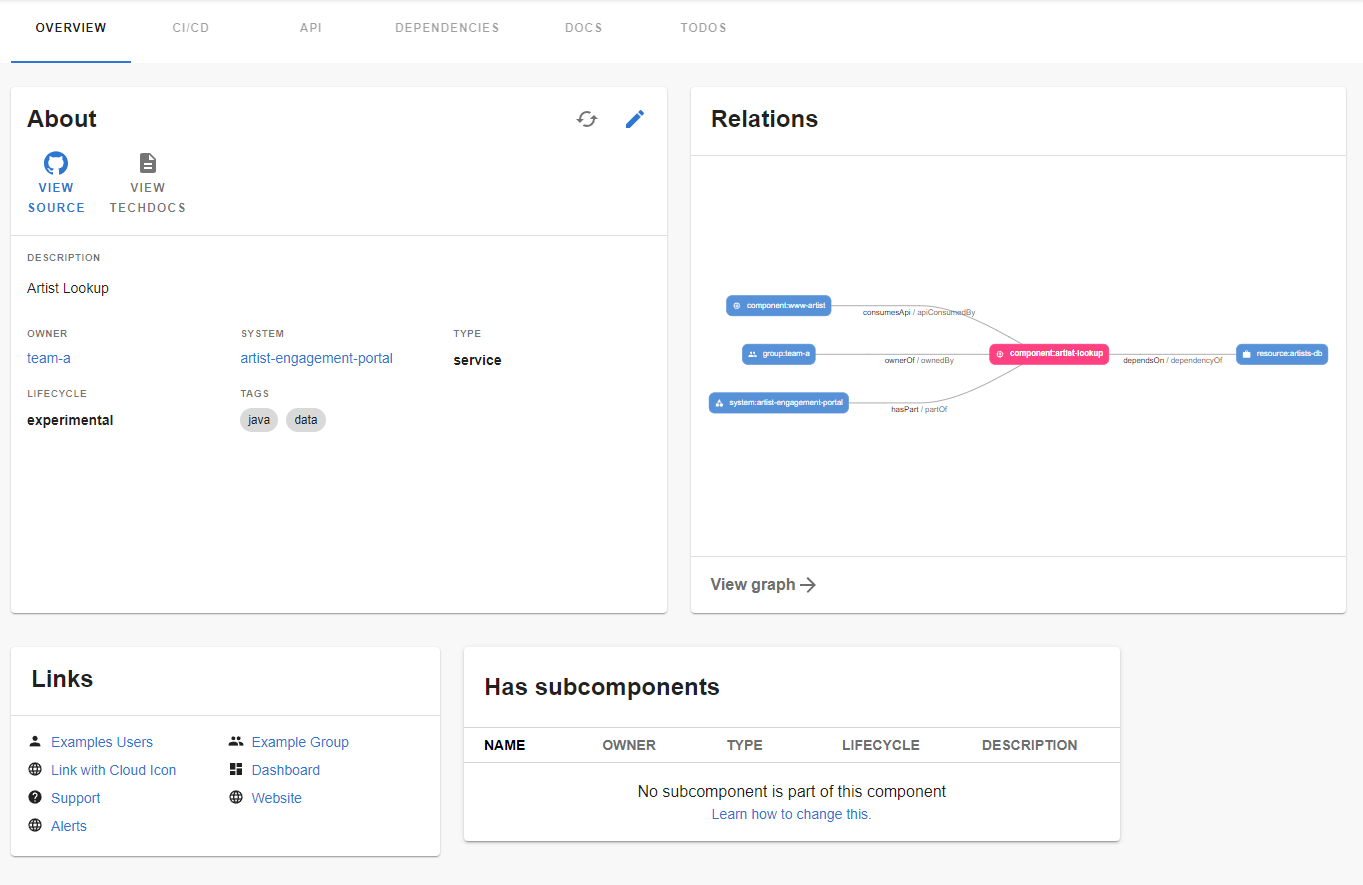
\includegraphics[width=\linewidth]{backstage_item_details}
        \caption{The Software Catalog from the Backstage Demo\parencite{backstagedemo}}
        \label{fig:catalog}
    \end{figure}

    Its content may be any combination of
    \begin{itemize}
        \item Teams with members
        \item Applications
        \item Infrastructure and platforms
        \item Most importantly, the relationships between those. These attributes are modelled, e.g. a application is owned by a team.
    \end{itemize}
    Data may be shown in a tabular fashion or may be shown as a relationship graph and the catalogue is searchable.
    An Engineer may bookmark its favourite items and its own resources are marked by 'owned'.

    In addition to the catalogue with its tabular overview, there is a details view.
    \begin{figure}
        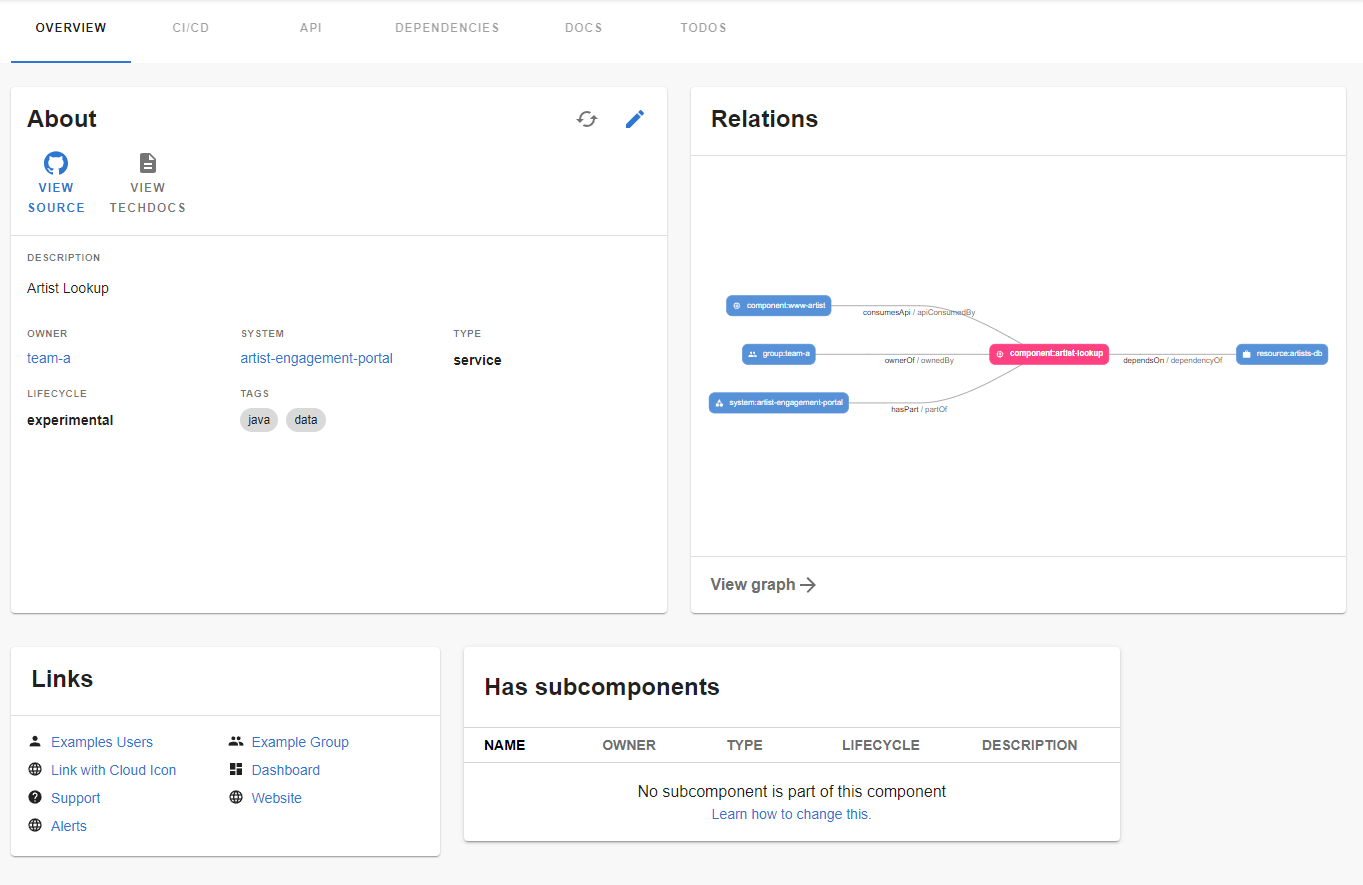
\includegraphics[width=\linewidth]{backstage_item_details}
        \caption{Details about an artifact}
        \label{fig:details}
    \end{figure}
    In the details view more attributes are shown for the chosen item from the overview.
    Depending on the kind of item, different attributes are shown.
    For an application, it may be its used resources, consumed and provided APIs and other subcomponents.
    For teams, the members are shown and its owned resources and its contact details.

    \subsubsection{Platform as a Product}
    In some implementations of an Internal Developer Portal, the catalogue is not merely a copy of an architecture database.
    In addition to the mentioned applications, platforms, organisational data and resources, there are other products
    of the teams shown.
    For example platform teams may offer support and consultation for their platform or area of expertise and advertise
    this service there.
    Some teams use the Internal Developer Platform to showcase code or libraries and thus create an inner-source community.
    In some cases, the whole lifecycle of a resource, from ordering, updating until removal are implemented or integrated
    in an Internal Developer Platform.


    \subsubsection{Golden Path}

    \subsubsection{Technical Documentation}

    \subsubsection{Expertise}

    \subsubsection{Extendability}


    \section{Situation at the SBB IT}
    The IT departement of the Swiss Federal Railywys (SBB) consists of around 1300 specialists and is responsible for
    700 applications\parencite{sbbitkennzahlen}.
    The application built and operated by this department are used for a wide range of use cases.
    For example, some applications are covering generic enterprise use cases such as human resource management, finance
    and controlling.
    Other software is specially built for mission-critical day-to-day operations of the railway such as the Rail Control
    System (RCS)\parencite{sbbrcs}.
    An SBB IT application may be a purchased products, is developed in-house or is a combination thereof which is sometimes called
    'customization'.

    \subsection{Internal Developer Platform}
    %bää TODO
    The SBB IT has for most of the core components, as defined by Richter et al\parencite{richteretal}, already one or more solutions
    in place.
    \begin{itemize}
        \item Application Configuration Management - is centered around the practice of GitOps\parencite{hashicorpvault}
        \item Infrastructure Orchestration - for example, SBB uses OpenShift since 2015\parencite{rhsbbopenshift}
        \item Environment Management - provided by OpenShift and CI/CD Pipelines
        \item Deployment Management - is provided by CI/CD pipelines built on Tekton and ArgoCD\parencite{sbbtekton}
        \item Role-Based Access Control - built-in in most of the SBB IT platforms
    \end{itemize}
    In addition, there are several other tools and applications used for the day-to-day operations and development.
    Most notable are the following
    \begin{itemize}
        \item Development and operation are dependent on a Wiki Software for documentation and communication.
        \item An Enterprise Architecture Database contains the information about used technologies, platforms and
        \item dependencies, as modelled by the architects
        \item An IT Service Management Platform contains the data concerning team contact information and support groups for applications
        \item A Configuration Management Database contains data about used assets, resources and relations to applications
    \end{itemize}
    Thus, it could be argued, that the foundation for an Internal Developer Platform is in place, but there are two
    critical pieces missing.
    First, most of the components mentioned are only partially integrated with each other.
    % perhaps argue with different identifier, authorization things.
    Second, there is no central view to aggregate data contained in these applications and tools for the benefit of the DevOps engineers.

    \subsection{DevOps}
    In 2015 DevOps and a platform-as-a-service was first introduced in the SBB IT.
    The stated goals of these additions was to solve the rising complexity in operations and the perceived low velocity
    in responding to change\parencite{sbbdevops}.
    Four years later, a reorganisation brought a new operating model to the SBB IT, based on agile principles, DevOps and SAFe
    and created the role of the BizDevOps engineer\parencite{sbbagile}.
    Most pre-reorganisation roles such as an application engineer, operations manager, test engineer or a requirements engineer
    were converted to this BizDevOps Engineer role.
    Even some former business oriented roles are now called BizDevOps engineers and are integrated in this cross-functional
    teams.
    DevOps teams are now established, but they are stilll working mostly with tools from the organisation before.
    While the tools itself may be the state of the art in their fields, they weren't bought or built with an end-to-end
    integration in mind which would benefit a BizDevOps engineer.

    \subsection{Internal Developer Portal}
    Most BizDevOps teams of the SBB help themselves with some kind of organisation for links.
    For example, they have a Wiki page, which consists of all necessary links for operations, e.g. link to monitoring
    of their product,    link to the productive OpenShift project space or a link to the log data.


    \section{Method}
    %TODO Umfrage.


    \section{Conclusion}
    \pagebreak


    \section{List of Sources}

    \printbibliography[heading=none]


\end{document}